\documentclass{beamer} 

\usepackage[utf8]{inputenc}
\usepackage[T1]{fontenc}
\usepackage{graphicx}
\usepackage[serbian]{babel}
\usepackage{multicol}

\usetheme{Berlin}
\begin{document}


\title{Segmentacija i klasifikacija elemenata na stranici dokumenta}
\author{Stefan Nožinić \\
student II godine master studija računarskih nauka \\
Departman za matematiku i informatiku \\
Prirodno-matematički fakultet \\
Univerzitet u Novom Sadu. \\
Tip rada: seminarski rad \\
Mentor: \MakeLowercase{prof. dr} Miloš Radovanović
}

\frame{
\titlepage
}

% \frame{
% 	\frametitle{Uvod}
% 	\begin{itemize} 
% 		\item Cilj je učenje istraživačkog procesa kroz:
% 		\item Planiranje
% 		\item Implementaciju
% 		\item Evaluaciju
% 		\item Dokumentovanje 
% 		\item Prezentaciju rezultata
% 	\end{itemize}
% }


% \frame{
% 	\frametitle{Smernice za postavljanje hipoteze}
% 	\includegraphics[width=\textwidth]{png/hipoteza.png}
% }

\begin{frame}
	\frametitle{Motivacija}
	\begin{itemize}
		\item OCR
		\item Konverzija PDF u druge formate 
	\end{itemize}

\end{frame}


\begin{frame}
	\frametitle{Problem}
	% graphics - rendered document and its tree representation 
	\begin{columns}
		\begin{column}{0.5\textwidth}
			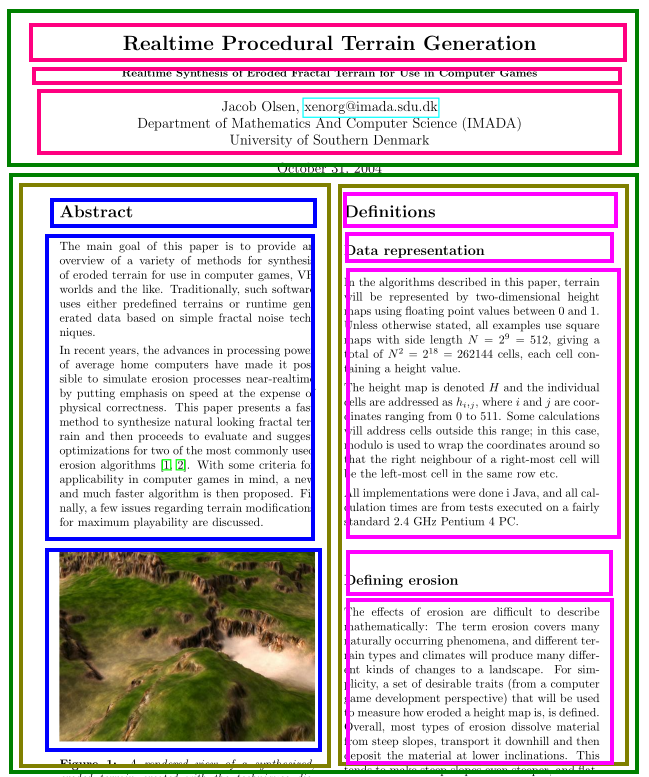
\includegraphics[width=\textwidth]{./png/segmented-doc.png}
		\end{column}
		\begin{column}{0.5\textwidth}
			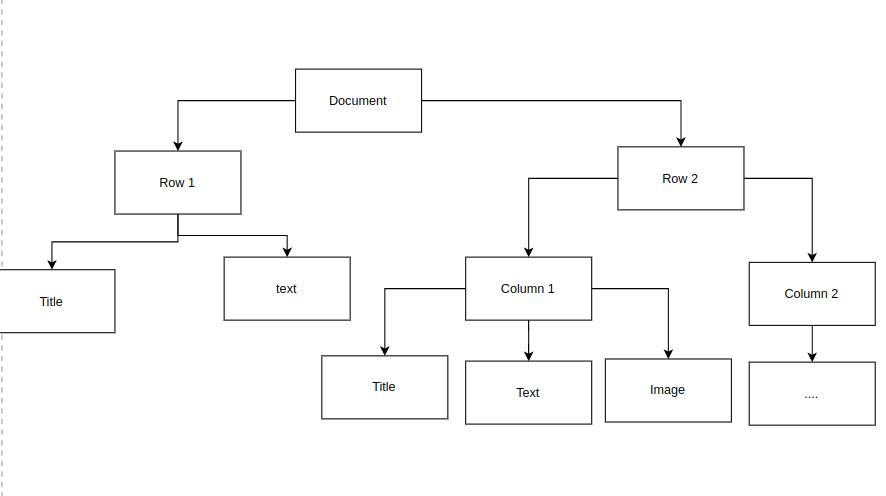
\includegraphics[width=\textwidth]{./png/tree.png}
		\end{column}
	\end{columns}
\end{frame}


\begin{frame}
	\frametitle{Reprezentacija celog sistema}
	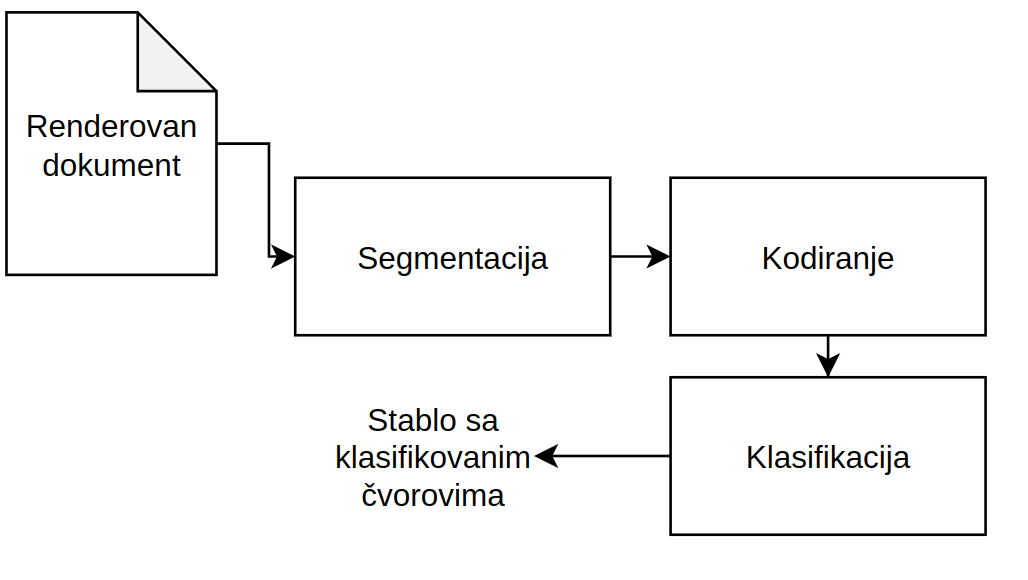
\includegraphics[width=\textwidth]{./png/system.png}
\end{frame}

\begin{frame}
	\frametitle{Ulazni podaci}
	\begin{itemize}
		\item Ulazni podaci su dokument reprezentovan kao sekvenca stranica koje su slike u RBG formatu.
		\item Dokument je prošao proces uklanjanja šumova ako je skeniran. 
	\end{itemize}
\end{frame}


\begin{frame}
	\frametitle{Izlazni podaci}
	\begin{itemize}
		\item Stablasta struktura
		\item Svaki čvor stabla ima dodeljeni region stranice ulaznog dokumenta. 
		\item Svaki čvor stabla ima labelu koja označava semantičko značenje tog dela dokumenta. 
	\end{itemize}
\end{frame}


\begin{frame}
	\frametitle{Segmentacija dokumenta}
	% show picture 
	\begin{columns}
		\begin{column}{0.5\textwidth}
			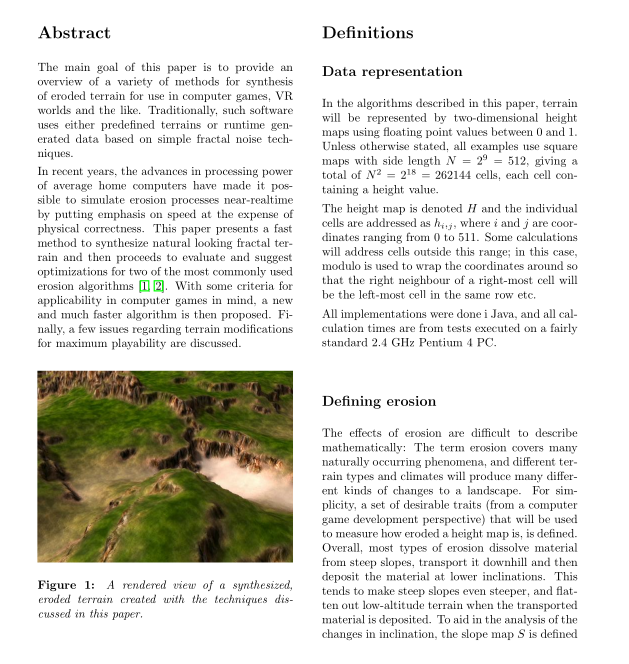
\includegraphics[width=\textwidth]{./png/segmentation-example.png}
		\end{column}
		\begin{column}{0.5\textwidth}
			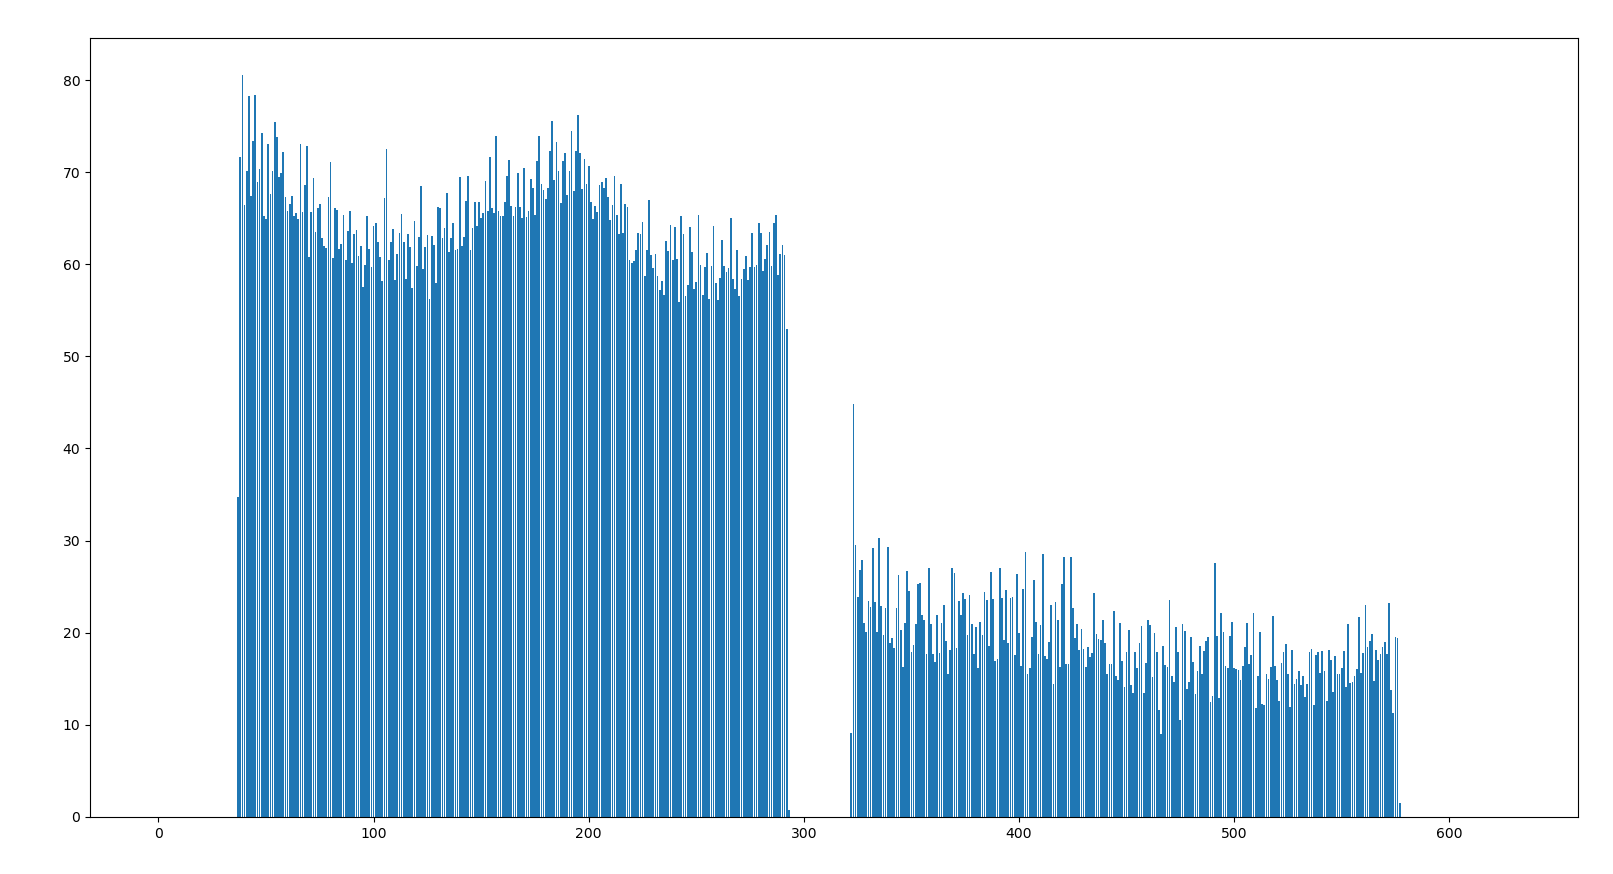
\includegraphics[width=\textwidth]{./png/segmentation-histogram.png}
		\end{column}
	\end{columns}
\end{frame}

\begin{frame}
	\frametitle{Proces klasifikacije}
	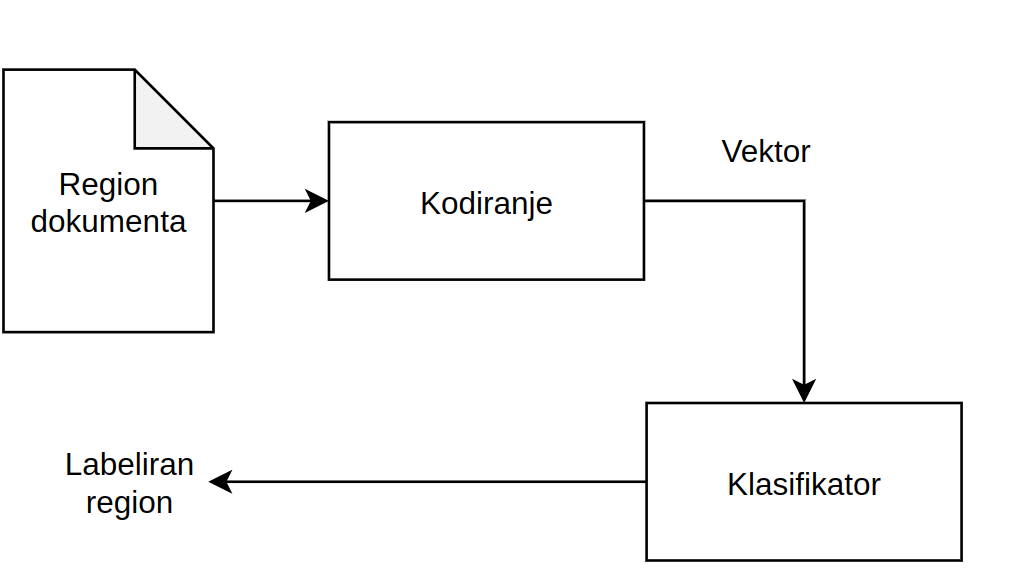
\includegraphics[width=\textwidth]{./png/classification.png}
\end{frame}

\begin{frame}
	\frametitle{Načini kodiranja}
	\begin{itemize}
		\item \texttt{simple}: Element je kodiran kao vektor [E.x, E.y, E.h, E.w], odnosno njegova pozicija i veličina su predstavljeni kao vektor.
		\item \texttt{img\_attrs}: Element je kodiran kao vektor:  [E.h * E.w, E.w / (E.h*E.w), E.h / E.w, prosečna vrednost piksela u E]
		\item \texttt{pixels}: [R(x,y) za svako (x,y) na slici R veličine LxL]
		\item \texttt{histogram}: Elementi su sume vrednosti piksela po kolonama i vrstama.
	\end{itemize}
\end{frame}


\begin{frame}
	\frametitle{Random decision forest}
	\begin{itemize}
		\item 100 stabala za klasifikaciju
		\item kreiranje svakog stabla bilo ograničeno sa maksimalnom dubinom od 2
		\item Kriterijum podele je bio vrednosti \textit{Gini} koeficijenta
	\end{itemize}
\end{frame}

\begin{frame}
	\frametitle{Neuronska mreža}
	\begin{itemize}
		\item jedan skriven sloj veličine 100 sa \textit{ReLU} aktivacionom funkcijom
		\item Trenirana standardnim BP algoritmom
	\end{itemize}
\end{frame}

\begin{frame}
	\frametitle{Rezultati}
	\begin{table}
		\begin{tabular}{rllr}
		 & Metod kodiranja & Klasifikator & Tačnost (\%)\\
		\hline
		1 & \texttt{histogram} & RF & 71.792\\
		2 & \texttt{img\_attrs} & RF & 72.034\\
		3 & \texttt{img\_attrs} & one rule & 63.153\\
		4 & \texttt{pixels} & NN & 38.451\\
		5 & \texttt{simple} & NN & 42.345\\
		6 & \texttt{simple} & RF & 70.422\\
		7 & \texttt{simple} & one rule & 63.216\\
		\end{tabular}
		\caption{Tačnost klasifikatora u odnosu na metode kodiranja}
	\end{table}

\end{frame}

\begin{frame}
	\frametitle{Zaključak}
	\begin{itemize}
		\item \textit{Random decision forest} je pokazao najbolje rezultate za izuzetno jednostavan metod kodiranja
		\item zadovoljavajući rezultati na 7 klasa.
		\item U Praktičnoj primeni, pogrešno klasifikovani elementi bi mogli da se modifikuju ručno.
		\item Neke pogrešno klasifikovane elemente ne treba smatrati podjednako lošim kao neke druge pogrešno klasifikovane elemente.
	\end{itemize}
\end{frame}

\begin{frame}
	\frametitle{Poboljšanja}
	\begin{itemize}
		\item Upotrebiti konvolucionu neuronsku mrežu.
		\item Proširiti skup za obuku.
		\item Određivanje matrice konfuzije za date klase.
	\end{itemize}
\end{frame}

\begin{frame}
	\frametitle{Pitanja}
	\begin{center}
		\huge{?}
	\end{center}
\end{frame}


\end{document}
